\documentclass[11pt]{article}
\usepackage{mypackages}
\begin{document}
\section{Policy Gradient Methods}

In the last section we discussed how to update the value function dynamically. Now, we instead consider learning a \textit{parameterized policy}, $\pi (a | s, \theta)$, for computing the probability of taking action $a$ in state $s$ under policy $\pi$ without estimating any value function. The advantage of using a parameterized policy is that it is possible to solve problems that consist of continuous state spaces\cite{policyGrad}, which is exactly what we are given in the Atari 2600 games. The parameterized policy is an function, for computing the probabilities for taking action $a$ in state $s$ using the parameters $\theta \in \mathbb{R}^{n}$. To improve the policy we update the weights, $\theta$, by computing the gradient of a differentiable \textit{performance measure}, $\rho$, with respect to the policy weights $\theta$, as we saw in section \ref{sec:eligibility_traces} with the value function, 
\begin{equation}
    \theta_{t + 1} = \theta_{t} + \alpha \nabla \rho (\theta_{t})
\end{equation}
The performance measure is a function used for evaluating the performance of the parameterized policy.
We will be using the following performance measure in this project,
\begin{equation}
    \rho(\theta) = \text{log} \pi (a | s, \theta)
\end{equation}
and by differentiate the right hand site we get,
\begin{equation}\label{eq:d_log}
    \nabla_{\theta} \text{ log} \pi (a | s, \theta) = \frac{\nabla \pi (a | s, \theta)}{ \pi (a | s, \theta)}
\end{equation}
which means the output of the performance measure is high if the probability is of taking action $a$ is low and vice versa.
\\ \\
The environments used in this project all have a continuous state space, and a discrete action space.
One challenge by using a parameterized policy combined with a discrete action space is that we need to ensure that the policy never becomes deterministic - that is $\pi (a|s,\theta) \in (0,1)$ $\forall s, a, \theta$. The reason that a deterministic policy will become a problem is that our agent don't use exploration for  exploring an environment, and that we will divide by 0 in equation \ref{eq:d_log}. A way to solve this problem is to use a numerical preference $h(s, a, \theta) \in \mathbb{R}$ for each state-action pair in each state. We can then use a function like the softmax function to make sure the probabilities for the actions are never 0 or 1,
\begin{equation}
    \pi(a | s, \theta) = \frac{e^{h(s,a,\theta)}}{\sum_{a} e^{h(s,a,\theta)}}
\end{equation}
and,
\begin{equation}
    \sum_{a} \pi (a | s, \theta) = 1
\end{equation}

\subsection{Actor-Critic Methods}

Actor-Critic methods are a type of policy gradient methods, that estimate both a state-value function $\hat{V}(s, \mathbf{w})$ and a parameterized policy $\pi(a | s, \theta)$. Actor-Critic methods use the value function to update the policy,

\begin{figure}[!h]
    \centering
    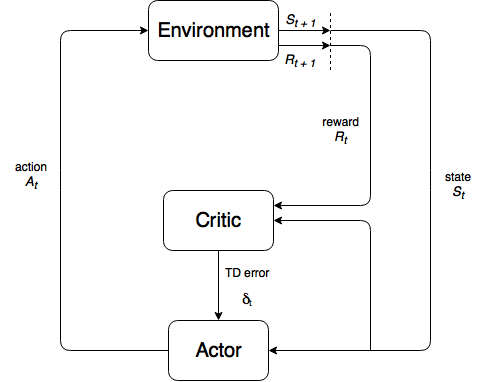
\includegraphics[scale = 0.5]{include/ActorCriticDiagram.png}
    \caption{A representation of the workflow in an Actor-Critic
    model. The environment sends a state and reward signal to both the actor and the critic. The critic compute the TD-error which is sent to the actor,
and then the actor perform a action and so forth.}
    \label{fig:actor-critic}
\end{figure}

The general idea in Actor-Critic methods is that the actor selects an action following policy $\pi$,

\begin{equation}
    A_{t} \sim \pi(\cdot | S_{t}, \theta_{t})
\end{equation}

Performing action $A$ results in a transition from state $S$ to state $S'$ and a corresponding reward $R$. The critic can use this information to evaluate the actor, which it does by computing the one-step td-error,
\begin{equation}
    \delta \leftarrow R + \gamma \hat{v} (S', \mathbf{w}) - \hat{v}(S, \mathbf{w})
\end{equation}
which make it is possible to update the parameters of the policy as,
\begin{equation}
\begin{split}
    \theta &\leftarrow \theta + \delta \nabla_{\theta} \text{ log } \pi(A | S, \theta)
\end{split}
\end{equation}
and the state-value function,
\begin{equation}
\begin{split}
    \mathbf{w} &\leftarrow \mathbf{w} + \delta \nabla_{\mathbf{w}} \hat{v}(S, \mathbf{w})
\end{split}
\end{equation}
where $\mathbf{w}$ is the weight vector used for the parameterized state-value function.
An advantage of using Actor-Critic methods is that the split into a actor and critic, reduces the variance of the function approximation, because the update step size for the policy parameters is defined relative to estimated value from critic.\cite{actCrit}


\subsection{Actor-Critic with Eligibility Traces}

In this project we using the \textit{Actor-Critic with eligibility traces}, which follow the workflow from figure \ref{fig:actor-critic}, and using eligibility traces for performing online updates of the weight vectors $\theta$ and $\mathbf{w}$. The general updating scheme for the eligibility vector $\mathbf{e}^{\mathbf{w}}$ is,
\begin{equation}
    \mathbf{e}^{\mathbf{w}} \leftarrow \lambda^{\mathbf{w}} \mathbf{e}^{\mathbf{w}} + \nabla_{\mathbf{w}} \hat{v}(S, \mathbf{w})
\end{equation}
and $\mathbf{e}^{\theta}$ as,
\begin{equation}
    \mathbf{e}^{\theta} \leftarrow \lambda^{\theta} \mathbf{e}^{\theta} + \nabla_{\theta} \text{log} \pi (A | S, \theta)
\end{equation}
where $\lambda$ discussed in section \ref{sec:td} is the discount rate, there represent how much the existing eligibility trace influence the update.
\\
The reason for using eligibility traces in Acotr-Critic methods is that it as elegant way for using the knowledge of how the gradients have changed in the last minor time period.

We have implemented Actor-Critic using Eligibility traces, and we follow this algorithm,\cite{RLbook}









%\printbibliography
%\bibliography{citations}
%\bibliographystyle{plain}
\end{document}